\documentclass[a4j,11pt,twocolumn]{jsarticle}

%\usepackage{multicol} %2段組み用
\usepackage{amsmath}  %alignなど数式関係で必要になることが多い.
%\usepackage{graphicx} %図の取り込みに利用.
\usepackage[dvipdfmx]{graphicx} %図の取り込みに利用.
\usepackage{url} %URLの表記に使う\urlコマンドに必要.
\usepackage{txfonts}
 %英文をTimes Romanのようなフォントにする.
 %通常のLaTeXのフォントにしたいときはこれをコメントアウトする.
\usepackage{algorithm,algorithmic} %algorithmとalgorithmic環境を利用するのに必要.
\usepackage{enumerate} %enumerate環境で項目を[Step 1.]のような形式に変更するのに利用.

\pagestyle{plain} %ページ番号のスタイル
\urlstyle{same} %\urlコマンドのフォント指定."tt", "rm", "sf", "same"(=使用中のフォント)

%%%%%%%%%%%%%%%%%%%%%%%%%%%%%% ↓テキスト幅,マージン,行間の調節
\textwidth     =  160mm %テキスト幅
\oddsidemargin = -7.5mm %左側のマージン
\textheight    =  230mm %テキストの高さ
\topmargin     =  -15mm %上のマージン
\renewcommand{\baselinestretch}{1.1} %行間を調節
%%%%%%%%%%%%%%%%%%%%%%%%%%%%%% ↑テキスト幅,マージン,行間の調節

%%%% ↓Change the style of itemize, enumerate, etc.
%%%% ↓(without space between items)
\makeatletter
\def\@listI{\leftmargin\leftmargini
    \topsep  \z@
    \parsep  \z@
    \itemsep \z@}
\let\@listi\@listI
\@listi
\def\@listii{\leftmargin\leftmarginii
    \labelwidth\leftmarginii\advance\labelwidth-\labelsep
    \topsep  \z@
    \parsep  \z@
    \itemsep \z@}
\def\@listiii{\leftmargin\leftmarginiii
    \labelwidth\leftmarginiii\advance\labelwidth-\labelsep
    \topsep  \z@
    \parsep  \z@
    \itemsep \z@}
\makeatother
%%%% ↑Change the style of itemize, enumerate, etc.

%%%% ↓algotithmic の \REQUIRE と \ENSURE の表記を変更する
\renewcommand{\algorithmicrequire}{\textbf{Input:}}
\renewcommand{\algorithmicensure}{\textbf{Output:}}
%%%% ↑algotithmic の \REQUIRE と \ENSURE の表記を変更する

\newcommand\coleq{\mathrel{\mathop:}=} %\coleqの定義(:=をきれいに出力する)

\begin{document}
\twocolumn[%
\begin{center}

 {\LARGE\bf
 自動車運搬船における貨物積載プランニングの席割問題}\\

\vspace{2mm}
 {\Large 竹田 陽} \\
 2021年7月9日
\vspace{1mm}

\end{center}
\begin{quote}
 {\bf Abstract.}
 Our research considers the situation in which cars are transported to several ports of various countries by a carrier ship for cars. Two stages of work called stowage planning and simulation planning are performed before loading a collection of cars onto a PCC (pure car carrier, PCC). The stowage planning stage considers assigning cars to one of the areas called holds, a few of which compose each level of the ship. The simulation planning stage places the cars assigned to each area in the stowage planning one by one considering the orientation of cars.
 In our research, as the first step of fully automating the stowage planning and simulation planning, the goal is to output stowage plans efficiently with a computer using mathematical optimization technology.
 We confirmed that we can get a good solution for small bookings. We also propose heuristic model to solve large bookings.
\end{quote}
\vspace{6mm}
]
\section{はじめに}
複数の港で荷物を船に積み, 複数の港で降ろす運搬船を考える. 積荷の種類としては燃料, 原料など多岐に渡るが本研究では自動車を運搬する船を考える. 一般的に自動車運搬船は, 自動車を船の一定間隔で区切られたホールドと呼ばれるスペースにどの自動車を何台割り当てるかを考える席割作業を行い, その後席割作業で割り当てられた自動車に対して向きと場所考慮して一台ずつ船内の領域に配置するシミュレーション作業をする. 現状自動車を輸送する会社はこの作業を人手で行っているが少なくとも席割作業に3時間, シミュレーション作業に4時間かかることから, 多大な人件費と時間をかける必要があり直前の追加注文等に対応が出来ないという問題点がある\cite{mitsui}. 本研究ではこの問題を解決するために, 席割作業とシミュレーション作業それぞれについて数理最適化技術を用いることで, コンピューター計算により短時間で有効な席割とシミュレーションを出力することを目標とする. ただし本稿では研究の第一段階として, 席割作業とシミュレーション作業のうち席割作業の自動化に対して検証した結果を記す.

本研究で扱う席割作業の概要について述べる. 様々な種類の車を港Aから港Bまで輸送するというような積載自動車の注文リストを受け取る. 注文リストを受け取ったプランナーと呼ばれる席割を作成する作業者は好ましい席割になるように, 注文の船内スペースへの割当を考える. 席割作成における前提条件について説明する. 例えば船内の特定の領域に積まれている自動車よりも奥に積まれている自動車が, ある港Cで降ろされて空きスペースが発生したとする. この場合次の港Dで積む自動車があればその自動車の積みやすさのために, 船内に積んだ自動車を奥側に詰めて手前の領域を確保するというような既に積まれた自動車の航海中の移動は原則しない. また自動車は全てのホールドに容易にアクセスすることは出来ない. 例えば本稿の実験で扱う自動車運搬船は12階構造の内5階のみに外部から自動車を入れるスロープがあり, 船内の奥側ホールドにアクセスしたい場合はそのホールドにアクセスする際に通過するホールドに十分な空きスペースがないとアクセスすることが出来ない.

本稿では第2章で席割問題に対する詳細な問題設定や, 本研究で扱う自動車輸送航海における専門用語について定義する.  第3章では注文に含まれる自動車一つ一つをどの領域に割り当てるかを最適化する数理モデルと, そのモデルに登場する本研究独自の制約や好ましい席割作成のための目的関数を説明する. 第4章では提案した数理モデルと商用ソルバーを用いて, 実際の過去の航海データを基に求解実験を行い,比較実験を行う.

\section{問題説明}
様々な国で複数の港を経由し, 自動車を輸送する運搬船を想定する. このとき乗用車100台を港Aから港B, トラック30台を港Cから港Dというような各注文を, 運搬船の階層毎に一定の広さで区切られたスペースへの割当を計画する.この作業を席割作業(stowage plan)\cite{stowage}という. 本稿では席割作業の自動化の初期段階として, 単純な船の構造データを用いて実験する. この章では一般的な船への自動車積載における専門用語の定義, 席割作業における入力情報や出力情報の説明をする.

\subsection{用語定義}
本研究で扱う船の航海等に関する専門用語の定義をする.

\begin{itemize}

\item 席割 \\
注文一つ一つを船のホールド割り当てる作業.

\item シミュレーション \\
席割で決まった自動車を一台ずつホールド内の領域に貼り付ける作業.

\item  プランナー \\
席割やシミュレーションを考える作業者.

\item  ギャング\\
港で自動車をホールドまで運転して積み降ろしをする作業者.

\item デッキ \\
船の内部の階層.

\item ホールド \\
各デッキ内を一定間隔の領域で仕切られた空間.

\item ランプ \\
上下デッキに移動するために各デッキの特定ホールドについているスロープ.

% \item 注文 \\
% 乗用車100台を港Aから港Bへ輸送, トラック30台を港Cから港Dへ輸送というような積載自動車の情報とそれらの積み地と揚げ地に関する情報.

\item 積み地 \\
注文における自動車を積む港.

\item 揚げ地 \\
注文における自動車を降ろす港.

\item  RT (revenue ton) \\
基準となる車一台の面積に対する各注文の車の面積の割合. 本研究ではこれを資源要求量として扱う\cite{stowage}.

\item ユニット数 \\
各注文に含まれる自動車の台数.

\end{itemize}

\subsection{入力情報}
本研究で扱う二種類の情報について述べる.
\begin{itemize}

\item 注文情報 \\
本稿では注文内に含まれる情報のうち注文番号, 積み地と揚げ地, ユニット数, 積載自動車のRT, 自動車の重量情報を扱う.

\item 船体情報 \\
輸送に使う船のデッキやホールド番号, 各ホールドへアクセスすために通るホールドや各ホールドの許容収容量などの船の内部構造に関する情報.

\end{itemize}

\subsection{出力}
入力情報を元に様々な条件を考慮して注文番号1番を3デッキ1ホールドに30台中30台割り当てる, 注文番号2番を2デッキ2ホールドに200台中40台割り当てる, というようなエクセルファイル形式の席割を出力する.


\section{定式化}
この章では各注文に含まれる自動車を, どのホールドに何台割り当てるかを最適化する数理モデルを提案する. モデルは,鵜川らによって提案されたモデル\cite{ukawa}に複数の制約を加えたものを示す.

\subsection{記号の定義}
本研究における変数と定数記号の定義をする. 本研究の変数の定義を表\ref{variable}に, 定数の定義を表\ref{const}に記載する. \\


\clearpage

\begin{table}[htb]
\caption{変数の定義}
\label{variable}
\begin{tabular}{cp{17em}} \hline
変数 & \hspace{0.55em}変数の説明  \\ \hline

$v_{ij}$ &
\begin{tabular}{l}
注文$j$をホールド$i$に$n$台($0 \leq n \leq u_j$) \\
割り当てるとき$v_{ij} = n$ \\
\end{tabular} \\ \hline

$x_{ij}$ &
\begin{tabular}{l}
注文$j$をホールド$i$に割り当てるとき \\
$x_{ij} = 1$ \\
そうでないとき$x_{ij} = 0$ \\
\end{tabular} \\ \hline

$n_{i}$ &
\begin{tabular}{l}
ホールド$i$の残容量が$b'_i$のとき \\
$n_{i} =  b'_i$ \\
\end{tabular} \\ \hline

$c_{ij}$ &
\begin{tabular}{l}
ホールド$i$に大きい注文$j$を100台以下 \\
に分割して積むとき$c_{ij} = 1$ \\
そうでないとき$c_{ij} = 0$ \\
\end{tabular} \\ \hline

$c_{i_1i_2j}^1$ &
\begin{tabular}{l}
ホールドペア$(i_1, i_2)$に \\
1.大きい注文$j_1$を分割して積むとき \\
$c_{i_1i_2j_1}^1 = p_{\rm{large}}^{\rm{c1}}$ \\
2.小さい注文$j_2$を分割して積むとき \\
$c_{i_1i_2j_2}^1 = p_{\rm{small}}^{\rm{c1}}$ \\
3.それ以外のとき$c_{i_1i_2j}^1 = 0$ \\
\end{tabular} \\ \hline

$c_{i_1i_2j}^2$ &
\begin{tabular}{l}
ホールドペア$(i_1, i_2)$に \\
分割した大きい注文$j_1$を \\
1.隣のホールド同士に積むとき \\
$c_{i_1i_2j_1}^2 = n\_p_{\rm{large}}^{\rm{c2}}$ \\
2.同デッキの隣ではないホールド同士 \\
に積むとき$c_{i_1i_2j_2}^2 = s\_p_{\rm{large}}^{\rm{c2}}$ \\
分割した小さい注文$j_2$を \\
3.隣のホールド同士に積むとき \\
$c_{i_1i_2j_2}^2 = n\_p_{\rm{small}}^{\rm{c2}}$ \\
4.同デッキの隣ではないホールド同士 \\
に積むとき$c_{i_1i_2j_2}^2 = s\_p_{\rm{small}}^{\rm{c2}}$ \\
5.それ以外のとき$c_{i_1i_2j}^2 = 0$ \\
\end{tabular} \\ \hline

$m_{it}$ &
\begin{tabular}{l}
ホールド$i$が港$t$で作業効率充填率を \\
超えているとき$m_{it} = 1$ \\
そうでないとき$m_{it} = 0$ \\
\end{tabular} \\ \hline

$m_{ijt}$ &
\begin{tabular}{l}
港$t$で注文$j$をホールド$i$から積み降ろ \\
しを行う際, $n$個の通過ホールドで作業効 \\
率充填率を超えそこを$v$台車が通るとき \\
$m_{ijt} = v n$ \\
\end{tabular} \\ \hline

\end{tabular}
\end{table}

\newpage

\begin{table}[htb]
\begin{tabular}{cp{17em}} \hline

$k_{it}^1$ &
\begin{tabular}{l}
ホールド$i$が港$t$で許容充填率を超えて \\
いるとき$k_{it}^1= 1$ \\
そうでないとき$k_{it}^1 = 0$ \\
\end{tabular} \\ \hline

$k_{it}^2$ &
\begin{tabular}{l}
ホールド$i$の残容量が1RTを$b'_i$超えて \\
いるとき$k_{it}^2 = b'_i$ \\
\end{tabular} \\ \hline

$k_{it}^3$ &
\begin{tabular}{l}
ホールド$i$が港$t$で許容充填率を超えて \\
それよりの奥のホールドの中で1RTを \\
超えたホールド残容量が$b'_i$のとき \\
$k_{it}^3 = p^k b'_i$ \\
\end{tabular} \\ \hline

$y_{it}^{\rm{keep}}$ &
\begin{tabular}{l}
ホールド$i$の中で港$t$を通過する注文が\\ あるとき$y_{it}^{\rm{keep}} = 1$\\
そうでないとき$y_{it}^{\rm{keep}} = 0$ \\
\end{tabular} \\ \hline

$y_{it_1t_2}$ &
\begin{tabular}{l}
ホールド$i$の中で港$t_1$で積んで港$t_2$で降ろす\\
注文があるとき$y_{it_1t_2} = 1$ \\
そうでないとき$y_{it_1t_2} = 0$ \\
\end{tabular} \\ \hline

$z_{it_1t_2}$ &
\begin{tabular}{l}
ホールド$i$の中で港$t_2$を通過する注文があり\\港$t_2$で降ろす注文の中に港$t_1$ \\
で積んだ注文があるとき$z_{i_1i_2t_1t_2} = 1$ \\
そうでないとき$z_{it_1t_2} = 0$ \\
\end{tabular} \\ \hline

$y_{i_1i_2t}^{\rm{load}}$ &
\begin{tabular}{l}
隣接ホールドペア$(i_1, i_2)$の中で港$t$で積む\\
注文があるとき$y_{i_1i_2t}^{\rm{load}} = 1$ \\
そうでないとき$y_{i_1i_2t}^{\rm{load}} = 0$ \\
\end{tabular} \\ \hline

$y_{i_1i_2t}^{\rm{keep}}$ &
\begin{tabular}{l}
隣接ホールドペア$(i_1, i_2)$の中で港$t$を通過する\\注文が
あるとき$y_{i_1i_2t}^{\rm{keep}} = 1$ \\
そうでないとき$y_{i_1i_2t}^{\rm{keep}} = 0$ \\
\end{tabular} \\ \hline

$y_{i_1i_2t}^{\rm{dis}}$ &
\begin{tabular}{l}
隣接ホールドペア$(i_1, i_2)$の中で港$t$で降ろす\\
注文があるとき$y_{i_1i_2t}^{\rm{dis}} = 1$ \\
そうでないとき$y_{i_1i_2t}^{\rm{dis}} = 0$ \\
\end{tabular} \\ \hline

$z_{i_1i_2t}^1$ &
\begin{tabular}{l}
隣接ホールドペア$(i_1, i_2)$の中で港$t$を通過する\\注文と積む注文があるとき \\
$z_{i_1i_2t}^1 = 1$ \\
そうでないとき$z_{i_1i_2t}^1 = 0$ \\
\end{tabular} \\ \hline

$z_{i_1i_2t}^2$ &
\begin{tabular}{l}
隣接ホールドペア$(i_1, i_2)$の中で港$t$を通過する\\注文と降ろす注文があるとき \\
$z_{i_1i_2t}^2 = 1$ \\
そうでないとき$z_{i_1i_2t}^2 = 0$ \\
\end{tabular} \\ \hline

\end{tabular}
\end{table}

\clearpage

\begin{table}[htb]
\caption{定数の定義}
\begin{tabular}{cp{17em}} \hline
\label{const}
定数 & \hspace{0.55em}定数の説明  \\ \hline

$T$ &
\begin{tabular}{l}
港の集合
\end{tabular} \\ \hline

$T^{\rm{c}}$ &
\begin{tabular}{l}
チェックポイント港の集合
\end{tabular} \\ \hline

$L$ &
\begin{tabular}{l}
積み地の集合
\end{tabular} \\ \hline

$D$ &
\begin{tabular}{l}
揚げ地の集合
\end{tabular} \\ \hline

$K$ &
\begin{tabular}{l}
船のデッキの集合
\end{tabular} \\ \hline

$J$ &
\begin{tabular}{l}
注文の集合
\end{tabular} \\ \hline

$J^{\rm{large}}$ &
\begin{tabular}{l}
ユニット数100台以上の大きい注文の集合
\end{tabular} \\ \hline

$J^{\rm{small}}$ &
\begin{tabular}{l}
ユニット数100台以下の小さい注文の集合
\end{tabular} \\ \hline

$J_{t}^{\rm{load}}$ &
\begin{tabular}{l}
港$t$で載せる注文の集合
\end{tabular} \\ \hline

$J_{t}^{\rm{keep}}$ &
 \begin{tabular}{l}
港$t$を通過する注文の集合
\end{tabular} \\ \hline

$J_{t}^{\rm{dis}}$ &
\begin{tabular}{l}
港$t$で降ろす注文の集合
\end{tabular} \\ \hline

$J_{t}^{\rm{lk}}$ &
\begin{tabular}{l}
$J_{t}^{\rm{load}}$と$J_{t}^{\rm{keep}}$の和集合
\end{tabular} \\ \hline

$J_{t}^{\rm{ld}}$ &
\begin{tabular}{l}
$J_{t}^{\rm{load}}$と$J_{t}^{\rm{dis}}$の和集合
\end{tabular} \\ \hline

$I$ &
 \begin{tabular}{l}
船のホールドの集合
\end{tabular} \\ \hline

$I^{\rm{lamp}}$ &
\begin{tabular}{l}
ランプがついているホールドの集合
\end{tabular} \\ \hline

$ I^{\rm{next}}$ &
\begin{tabular}{l}
隣同士のホールドペアの集合
\end{tabular} \\ \hline

$ I^{\rm{same}}$ &
\begin{tabular}{l}
同一デッキ内にあるホールドペアの集合
\end{tabular} \\ \hline

$ \overline{I}$ &
\begin{tabular}{l}
隣接しているホールドペアの集合
\end{tabular} \\ \hline

$ I^{\rm{num}}$ &
 \begin{tabular}{l}
船のホールド総数
\end{tabular} \\ \hline

$I_{k}^{\rm{deck}}$  &
 \begin{tabular}{l}
デッキ$k$のホールドの集合
\end{tabular} \\ \hline

$I_{i}^{\rm{back}}$  &
 \begin{tabular}{l}
ホールド$i$よりも奥のホールドの集合
\end{tabular} \\ \hline

$I^{*}_i$ &
 \begin{tabular}{l}
ホールド$i$に辿り着くまでに通る \\ ホールドの集合
\end{tabular} \\ \hline

$u_{j}$ &
\begin{tabular}{l}
注文$j$に含まれる自動車の台数
\end{tabular} \\ \hline

$g_{j}$ &
\begin{tabular}{l}
注文$j$における自動車一台の重量
\end{tabular} \\ \hline

$a_{j}$ &
\begin{tabular}{l}
注文$j$における自動車一台のRT
\end{tabular} \\ \hline

$b_{i}$ &
\begin{tabular}{l}
ホールド$i$の総面積
\end{tabular} \\ \hline





\end{tabular}
\end{table}

\newpage

\begin{table}[htb]
\begin{tabular}{cp{17em}} \hline

  $\delta_{i}^{\rm{h}}$ &
  \begin{tabular}{l}
  船の横方向のホールド$i$の重み
  \end{tabular} \\ \hline

  $d^{\rm{s}}$ &
  \begin{tabular}{l}
最大許容デッドスペース
  \end{tabular} \\ \hline

  $f_1^{\rm{h}}$ &
  \begin{tabular}{l}
  船の横方向の後方許容値
  \end{tabular} \\ \hline

  $f_2^{\rm{h}}$ &
  \begin{tabular}{l}
  船の横方向の前方許容値
  \end{tabular} \\ \hline

  $\delta_{i}^{\rm{v}}$ &
  \begin{tabular}{l}
  船の縦方向のホールド$i$の重み
  \end{tabular} \\ \hline

  $f^{\rm{v}}$ &
  \begin{tabular}{l}
  船の縦方向の上方許容値
  \end{tabular} \\ \hline

  $ \overline{q}_{i}$ &
  \begin{tabular}{l}
  ホールド$i$における許容充填率
  \end{tabular} \\ \hline

  $ \overline{q}^{\rm{s}}_{i}$ &
  \begin{tabular}{l}
  ホールド$i$における作業効率充填率
  \end{tabular} \\ \hline

  $\delta_i^{\rm{n}}$ &
  \begin{tabular}{l}
  ホールド$i$の残RT利得
  \end{tabular} \\ \hline

  $p^{\rm{c}}$ &
  \begin{tabular}{l}
  変数$c_{ij}$のペナルティ重み
  \end{tabular} \\ \hline

  $H_i^{\rm{h}}$ &
  \begin{tabular}{l}
  ホールド$i$の高さ
  \end{tabular} \\ \hline

  $H_j^{\rm{v}}$ &
  \begin{tabular}{l}
  注文$j$に含まれる自動車の高さ
  \end{tabular} \\ \hline

  $p^{\rm{c}}$ &
  \begin{tabular}{l}
  変数$c_{ij}$のペナルティ重み
  \end{tabular} \\ \hline

  $p^{\rm{k}}$ &
  \begin{tabular}{l}
  変数$k_{it}^3$のペナルティ重み
  \end{tabular} \\ \hline

  $p^{\rm{z}}$ &
  \begin{tabular}{l}
変数$z_{it_1t_2}$のペナルティ重み
  \end{tabular} \\ \hline

  $p^{\rm{z}}_1$ &
  \begin{tabular}{l}
変数$z_{i_1i_2t_1t_2}^1$のペナルティ1
  \end{tabular} \\ \hline

  $p^{\rm{z}}_2$ &
  \begin{tabular}{l}
  変数$z_{i_1i_2t_1t_2}^2$のペナルティ
  \end{tabular} \\ \hline

  $p_{\rm{large}}^{\rm{c1}}$ &
  \begin{tabular}{l}
  大きい注文の変数$c_{i_1i_2j}^1$のペナルティ
  \end{tabular} \\ \hline

  $p_{\rm{small}}^{\rm{c1}}$ &
  \begin{tabular}{l}
  小さい注文の変数$c_{i_1i_2j}^1$のペナルティ
  \end{tabular} \\ \hline

  $p_{\rm{large}}^{\rm{sc2}}$ &
  \begin{tabular}{l}
  大きい注文の変数$c_{i_1i_2j}^2$の緩和量1
  \end{tabular} \\ \hline

  $p_{\rm{large}}^{\rm{nc2}}$ &
  \begin{tabular}{l}
  大きい注文の変数$c_{i_1i_2j}^2$の緩和量2
  \end{tabular} \\ \hline

  $p_{\rm{small}}^{\rm{sc2}}$ &
  \begin{tabular}{l}
小さい注文の変数$c_{i_1i_2j}^2$の緩和量1
  \end{tabular} \\ \hline

  $p_{\rm{small}}^{\rm{nc2}}$ &
  \begin{tabular}{l}
小さい注文の変数$c_{i_1i_2j}^2$の緩和量2
  \end{tabular} \\ \hline

  $w_1$ &
  \begin{tabular}{l}
  目的関数(a)の重み
  \end{tabular} \\ \hline

  $w_2$ &
  \begin{tabular}{l}
目的関数(b)の重み
  \end{tabular} \\ \hline

  $w_3$ &
  \begin{tabular}{l}
  目的関数(c)の重み
  \end{tabular} \\ \hline

  $w_4$ &
  \begin{tabular}{l}
目的関数(d)の重み
  \end{tabular} \\ \hline

  $w_5$ &
  \begin{tabular}{l}
  目的関数(e)の重み
  \end{tabular} \\ \hline

  $w_6$ &
  \begin{tabular}{l}
  目的関数(f)の重み
  \end{tabular} \\ \hline

\end{tabular}
\end{table}


\clearpage
\subsection{制約}
本研究で扱う制約の中で一般的な割当問題とは異なる独自の制約について説明する.

\textgt{(a)自動車移動経路に関する制約} \\
 ある港で注文が運搬船内の特定のホールドにおいて積み降ろしがあるとき,自動車がホールドへ到達するためには船の入り口とホールドの間で通過する任意のホールドに対して,自動車が通るための道を作る必要がある.従って,本研究では各ホールドに対して自動車の移動通路が十分確保出来る許容充填率を定義し,任意の港で各ホールドに注文を積むときや各ホールドから注文を降ろすときには,入口とそのホールドの間で通過する全てのホールドで現状の充填率が許容充填率以下であることが必要である.

\textgt{(b)貨物の重量バランスに関する制約} \\
 運搬船で自動車を運ぶ際に船の外側へ自動車を詰め込みすぎると船が航海の途中で割れてしまったり,船の上方へ自動車を詰め込みすぎると船が傾いたときにバランスを崩しそのまま横転してしまうというような問題がある[3].本研究ではこの問題を考慮するため,過去10回分の航海データを解析することによりその航海内での運搬船の重量バランスを数値化した.その結果得られた10回分の航海データの中で最も重量バランスが偏ったときを閾値とし,運搬船の上下方向と前後方向それぞれに対して,各港において運搬船からで降ろす注文を全て降ろしたとき,または港で載せる注文を全て載せたときについて重量バランスが閾値を超えてしまうような荷物の割当を禁止する.

\textgt{(c)注文の分割ルールを守る} \\
 最初に注文を100台以下の小さい注文と100台以上500台以下の大きい注文と500台以上の巨大な注文に分割する. 小さい注文についてはモデルSP1-1と同じようにギャングの効率を考え分割をしない. 大きい注文に関しては一つのホールドでは全ての自動車が入りきらないことがあるので, 1つのデッキ内に注文に含まれる全ての自動車が収まるようにする. 巨大な注文についてはユニット数が500台以上1000台以下の場合には二等分, 1000台以上1500台以下の場合には三等分し別々の注文としてから大きい注文に加える. また等分した注文は別々のデッキに載せ, 大きい注文と同様に1つのデッキ内に全ての自動車が収まるようにする.

\textgt{(d)船内の高さに関する制約} \\
 それぞれのホールドには高さがあるため,積載する自動車の高さがホールドの高さを超えない必要がある.

\subsection{目的関数}
本研究で扱う目的関数について述べる. 席割に関するプランナーとの意見交換や,実際の席割作業を体験することで,プランナーは席割を考える上で注文の降ろし間違えが起こらないような席割を第一に目指していることが推測された.本研究では,このような席割を実現するために3つの目的関数のパラメータを提案する.

\textgt{(a)一つのホールド内の降ろし地を揃える} \\
 ある港においてホールドから注文を降ろす場合,同じホールド内に降ろし地の異なる注文が複数存在していると注文の降ろし間違いが発生する可能性がある. 本研究では降ろし地において注文を各ホールド内で降ろすときに,その降ろし地を通過する注文があるときにペナルティが発生する.またこのとき更に降ろす注文の中で載せた港が異なる注文が複数含まれていたとする.この場合,席割作業の次にホールド内のどの領域に自動車を一台ずつ詰めていくのかを考える際,手配師は降ろし間違えを防ぐため降ろし地が同じ注文は出来るだけホールド内の一つの領域に行き渡るようにホールド内のスペース配分などを考慮しなければならない.このような手配師の負担を考え,この場合は降ろす注文の中に含まれる相異なる載せ地の分だけ更にペナルティが加算される.

\textgt{(b)船内で注文の積み降ろし地を揃える} \\
 ギャング達とのヒアリングで,積み間違いや降ろし間違いを防ぐためになるべく積み降ろし地が同じ注文は船内の同じところで固めておきたいという要望があった.本研究ではこの要望に応えるために隣接ホールドペアを用意した.隣接ホールドペアとは,例えば4デッキの3ホールドと4デッキの2ホールドのような隣り合ったホールド同士のペアと, 5デッキの3ホールドと6デッキの1ホールドのようなスロープで繋がったホールド同士のペアのことである.このホールドペアの表を用いて各隣接ホールドペアに対して目的関数(a)と同様に,異なる積み降ろし地の数だけペナルティが加算される.

\textgt{(c)作業効率充填率を考慮する} \\
 ある港で注文の積み降ろしのために自動車をホールドから出すときやホールドに自動車を入れるときに,そのホールドと入口の間で通過するホールドの中にはその港を通過する注文が一定数割り当てられている.この注文がある一定量以上の場合,プランナーはそのホールドを自動車が通れるための道を作る必要がありホールド内における自動車のスペース配分を考える必要がある.またギャングは作られた道に自動車を通さなければいけないため,自動車の移動に慎重になり全体の作業効率が落ちる可能性が高い.本研究ではこのように作業効率が落ちないための各ホールド毎の作業効率充填率を設定し,これを上回ったホールドを自動車が通過する場合,通過する自動車の台数毎にペナルティが発生する.

\textgt{(d)デッドスペースを作らない} \\
 注文の合計資源要求量が船の合計収容量より十分小さい場合, 特定のホールドに空きスペースが出来る. このスペースが入口付近にあれば追い積みという港での突然の追加注文を積むことに対応出来るが, 空きスペースが出来たホールドに到達するまでに通るホールドが許容充填率を上回っている場合は, このスペースに追い積みをすることは出来ない. このような空きスペースのことをデッドスペースと言う. 目的関数(d)ではランプで繋がった船のホールドが許容充填率を超え特定デッキ間の移動ができない状態になったとき, そのホールドよりも奥にあるホールドの中で, 指定された最大許容デッドスペースよりも大きいデッドスペースがあるホールドが存在するときに大きいペナルティが発生する. \\

\textgt{(e)残容量をなるべく入口付近に寄せる} \\
 船の入口に近いホールドにまだ自動車を入れることのできるスペースがあると船への追い積みに対応できる. また, 研究で扱う船は追い積みに対応しやすい5デッキに残容量をなるべく残したいとのプランナーから要望があった. 目的関数(e)では, 積載自動車を全て積み終わる最後の積み地をチェックポイントとし, チェックポイントで5デッキや入口に近いホールドに対して残容量が多いほど全体目的関数のペナルティを減らす利得が発生する. \\

\subsection{定式化}
目的関数と制約の定式化を以下に示す.



\begin{align}
  &\textrm{min} \hspace{0.4em} {w_1 p^{\rm{z}} \sum_{i \in I} \sum_{t_1 \in L}  \sum_{t_2 \in D} {z_{it_1t_2}}} \notag \\
&\hspace{0.85em} + {w_2 \sum_{i_1 \in I} \sum_{i_2 \in I} (p_1^{\rm{z}} \sum_{t_1 \in L} {z_{i_1i_2t_1}^1} + p_2^{\rm{z}} \sum_{t_2 \in D} {z_{i_1i_2t_2}^2} )} \notag \\
&\hspace{0.85em} + {w_3 \hspace{0.1em} \sum_{i \in I} \sum_{j\in J} \sum_{t \in T}  {m_{ijt}} }
+ {w_4 \hspace{0.1em} p^{\rm{k}} \sum_{i \in I^{\rm{lamp}}} \sum_{t \in L} {k_{it}^3}} \notag \\
&\hspace{0.85em} - {w_5 \hspace{0.1em} \sum_{i \in I} \sum_{t \in T^{\rm{c}}} \delta_i^{\rm{n}} {n_{it}}}  \\ %ここまで目的関数
&\textrm{s.t.} \hspace{0.5em} x_{ij} \in \{ 0 , 1 \}, {y_{it}^{\rm{keep}}} \in \{ 0 , 1 \}, \notag \\
&\hspace{1.5em}  {y_{it_1t_2}} \in \{ 0 , 1 \}, z_{it_1t_2} \in \{ 0 , 1 \},  {y_{i_1i_2t}^{\rm{load}}} \in \{ 0 , 1 \}, \notag \\
&\hspace{1.5em}  {y_{i_1i_2t}^{\rm{keep}}} \in \{ 0 , 1 \}, {y_{i_1i_2t}^{\rm{dis}}} \in \{ 0 , 1 \}, {m_{it}} \in \{ 0 , 1 \}, \notag \\
&\hspace{1.5em}{k^1_{it}} \in \{ 0 , 1 \}, {k^2_{it}} \in \{ 0 , 1 \}, \notag \\
&\hspace{1.5em} 0 \leq z_{i_1i_2t}^1, 0 \leq z_{i_1i_2t}^2, 0 \leq m_{ijt}, 0 \leq k^3_{it}, 0 \leq n_{it}, \notag \\
&\hspace{1.5em} 0 \leq v_{ij} \leq u_j, \hspace{1.85em} \forall i \in I, \forall j \in J, \forall t \in T. \\
&\hspace{1.0em} \sum_{i \in I} x_{ij} = 1, \hspace{8.34em} j \in J^{\rm{small}}. \\
&\hspace{1.0em} \sum_{i \in I} {\hspace{0.6em}v_{ij}} = u_j, \hspace{8.33em} j \in J. \\
&\hspace{1.0em} \sum_{j \in J} {\hspace{0.65em}a_{j}}{v_{ij}} \leq {b_{i}}, \hspace{8.7em} i \in I. \\
&\hspace{0.5em} \sum_{j \in {J_t}^{\rm{keep}}} \frac{a_{j} v_{ij}} {b_{i}} \geq \overline{q}_{i}^{\rm{s}} + {m_{it}}, \hspace{3.76em} i \in I, t \in T.
\end{align}


\newpage

\begin{align}
  &\hspace{0.8em} \sum_{i_2 \in {I_{i_1}^*}} {m_{i_2t} v_{i_1j}} \leq {m_{i_1jt}}, \hspace{2.4em} i_1 \in I, j \in J_{t}^{\rm{ld}}, t \in T. \\
  &\hspace{1.0em} \sum_{j \in J_{t}^{\rm{lk}}} \frac{a_{j} v_{ij}} {b_{i}} \leq k^1_{it} + \overline{q}_{i}, \hspace{3.85em} i \in I^{\rm{lamp}}, t \in L. \\
  &\hspace{1.0em} \sum_{j \in J_{t}^{\rm{lk}}} \frac{a_{j} v_{ij} + d^{\rm{s}}} {b_{i}}  \geq 1 - k^2_{it}  \hspace{3.28em} i \in I, t \in L. \\
  &\hspace{1.0em} \sum_{j_1\in {J_t}^{\rm{keep}}} \frac{a_{j_1} v_{i_1j_1}} {b_{i_1}} \leq \overline{q}_{i_2} + 1 - {x_{i_2j_2}}, \notag \\
  &\hspace{3.91em} i_1 \in {I_{i_2}^*}, i_2 \in I, j_2 \in J_{t}^{\rm{ld}}, t \in T. \\
  &\hspace{1.0em} \sum_{j \in J_{t}^{\rm{lk}}} a_j v_{ij}  \leq b_{i} - n_{it}, \hspace{3.37em} i \in I, t \in T^{\rm{c}}. \\
  &\hspace{1.0em} \sum_{i_2 \in I_{i_1}^{\rm{back}}} k^2_{i_2t} + I^{\rm{num}} (k^1_{i_1t} - 1) \leq  k^3_{i_1t}, \notag \\
  &\hspace{12.91em} i \in I^{\rm{lamp}}, t \in L. \\
  &\hspace{1.0em} \sum_{i_1 \in I_{k_{1}}^{\rm{deck}}} x_{i_1j} \sum_{i_2 \in I_{k_{2}}^{\rm{deck}}} x_{i_2j} \leq 0, \notag \\
  &\hspace{6.91em} j \in J^{\rm{large}}, k_1, k_2 \in K, k_1 \neq k_2. \\
  &\hspace{1.0em} \frac{v_{ij}} {u_j} \leq x_{ij}, \hspace{6.33em} i \in I, j \in J. \\
  &\hspace{1.0em} {f^{\rm{h}}_1} \leq {\delta_{i}^{\rm{h}}}{g_{j}} {v_{ij}} \leq f^{\rm{h}}_2, \hspace{1.5em} i \in I, j \in J_{t}^{\rm{keep}} \cup J_{t}^{\rm{lk}}, t \in T. \\
  &\hspace{1.0em} {\delta_{i}^{\rm{v}}}{g_{j}} {v_{ij}} \leq f^{\rm{v}}, \hspace{1.5em} i \in I, j \in J_{t}^{\rm{keep}} \cup J_{t}^{\rm{lk}}, t \in T. \\
  &\hspace{1.0em} {x_{ij}} \leq {y_{it}^{\rm{keep}}}, \hspace{4.11em} i \in I, j \in J_{t}^{\rm{keep}}, t \in T. \\
  &\hspace{1.0em} {x_{ij}} \leq {y_{it_1t_2}}, \hspace{1.61em} i \in I, j \in J_{t_1}^{\rm{load}} \cap J_{t_2}^{\rm{dis}}, {t_1},{t_2} \in T. \\
  &\hspace{1.0em} {z_{it_1t_2}} \leq {y_{it_2}^{\rm{keep}}} ,  \hspace{2.50em} i \in I, j \in J_{t_2}^{\rm{keep}}, t_1,t_2 \in T. \\
  &\hspace{1.0em} {z_{it_1t_2}} \leq {y_{it_1t_2}} ,  \hspace{3.49em} i \in I, j \in J_{t_2}^{\rm{keep}}, t_1,t_2 \in T. \\
&\hspace{1.0em} {y_{it_1t_2}} + y_{it_2}^{\rm{keep}} - 1 \leq {z_{it_1t_2}}, \hspace{1.79em} i \in I, t_1,t_2 \in T. \\
&\hspace{1.0em} {x_{i_1j}} + {x_{i_2j}} \leq 2{y_{i_1i_2t}^{\rm{load}}}, \hspace{1.71em} i_1, i_2 \in \overline{I}, j \in J_{t}^{\rm{load}}, t \in T. \\
&\hspace{1.0em} {x_{i_1j}} + {x_{i_2j}} \leq 2{y_{i_1i_2t}^{\rm{keep}}}, \hspace{1.64em} i_1, i_2 \in \overline{I}, j \in J_{t}^{\rm{keep}}, t \in T. \\
&\hspace{1.0em} {x_{i_1j}} + {x_{i_2j}} \leq 2{y_{i_1i_2t}^{\rm{dis}}}, \hspace{1.19em} i_1, i_2 \in \overline{I}, j \in J_{t}^{\rm{dis}}, t \in T. \\
&\hspace{1.0em} {y_{i_1i_2t}^{\rm{load}}} + y_{i_1i_2t}^{\rm{keep}} - 1 \leq {z_{i_1i_2t}^1}, \hspace{1.77em}  i_1, i_2 \in \overline{I}, t \in L. \\
&\hspace{1.0em} {y_{i_1i_2t}^{\rm{dis}}} + y_{i_1i_2t}^{\rm{keep}} - 1 \leq {z_{i_1i_2t}^2}, \hspace{1.58em}  i_1, i_2 \in \overline{I}, t \in D. \\
&\hspace{1.0em} \sum_{j \in J} \sum_{i \in I} H_j^{\rm{v}} {x_{ij}} \leq H_i^{\rm{h}},  \hspace{3.5em} i \in I, j \in J
\end{align}

\newpage


\section{計算実験}
鵜川らによる研究の数理モデルでは自動車の注文数や積み地や揚げ地の数の増加とともに制約や組合せが急速に増加してしまい,指定された時間内では十分に計算が進まない可能性が指摘されている.\cite{ukawa}

\subsection{解くことのできる問題例の規模}
注文数や港の数を変更した問題例をいくつか準備し,どの程度の規模の問題例ならばある程度の時間内で解けるのか調査を行った.
実験に用いるプログラムは Pythonを用いて実装し, 計算機はPowerEdge T320 (CPU: Intel(R) Xeon(R) CPU E5-1410 v2 (2.80 GHz, 10 M cache), RAM: 96 GB) を使用した. また,整数計画ソルバーとしてGurobi Optimizer (ver 9.0.0) を使用した.

表\ref{24hours}に実行可能解が初めて出力された計算時間と,計算を回して1時間後と24時間後の解の精度を示した.

結果より,注文数が250程度,港の数が3,4より少なければ,24時間以内にある程度の解を出力することが確認できた.
一方で,注文数が350の問題例に関しては,24時間後でも解の探索があまり進まなかった.

実際にはこれ以上の注文数を持つ問題例が多く存在しており,提案したモデルではより大規模な問題例を解くことは難しいと考えられる.

\section{ヒューリスティックモデル}
より大規模な問題例を現実的な時間で解くために,ヒューリスティックを用いた数理モデルを提案する.

\subsection{ホールドの統合}
本研究では,ホールドの数が43の運搬船を考えている.
実オペレーションでは,それぞれのホールドを個別で考えるのではなく,複数のホールドをある程度まとめて考えて作業を行っている.
そのため,各階においてスロープのついているホールドを境目として,2つのホールドのまとまりとして考える.

複数のホールドを1つのまとまりとして考えると,43のホールドを,17のまとまりに統合することができる.このまとまりをセグメントと呼び,具体的な統合については
図\ref{fig1}に示す.

\begin{figure}[htbp]
 \centering
 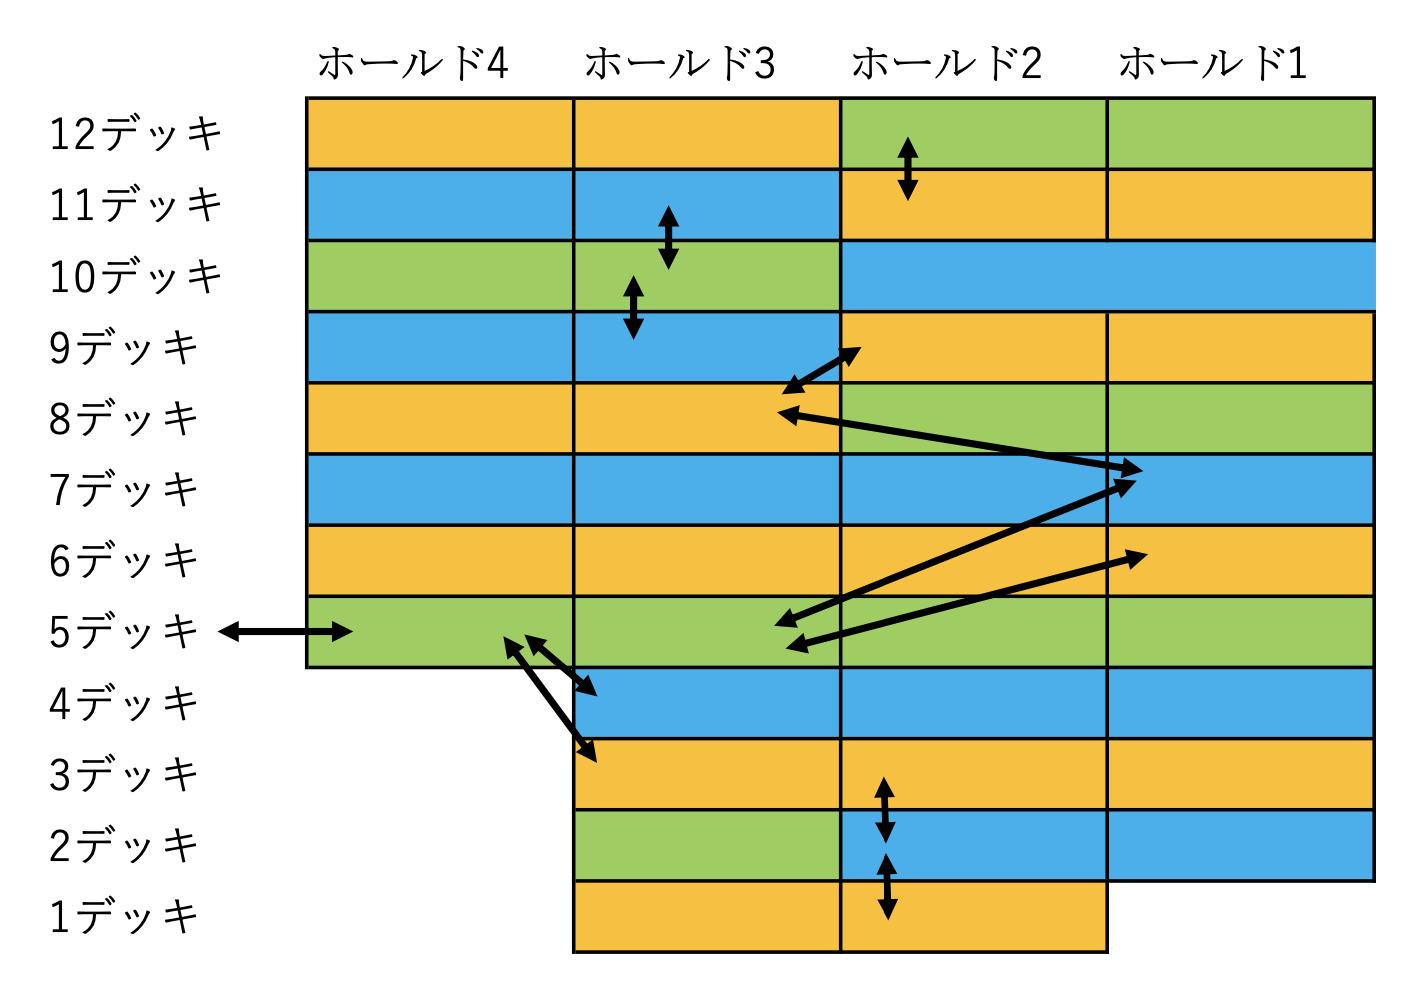
\includegraphics[width=0.9\linewidth]{segment.png}
 \caption{統合後のホールドを色付けしたもの}
 \label{fig1}
\end{figure}

\subsection{解の表現方法}
鵜川らによる研究の数理モデル\cite{ukawa}では,ホールドに注文を何台割り当てる,という連続的な解の表現方法を用いていた.
ヒューリスティックモデルでは,このような連続的な解表現方法を用いず,注文のセグメントへの割当のみを最適化し,詳細な車両の積載は決め打ちのルールを基に行っていく.
積載のルールは,ホールドの積載可能量,許容充填率などを満たすように設計を行っていく.

\section{局所探索法}
局所探索法とは, ある解に少しの変更を加え得た近傍解が元の解よりも良い解である場合に, 変更後の解に移動するという操作を良い解が見つからなくなるまで繰り返す方法である.
変形を加える操作を近傍操作と呼び, 近傍内に改善解を持たない解を局所最適解と呼ぶ.

\subsection{初期解の生成}
各セグメントに対して,すべての注文をランダムに割り当てたものを用いる.

\subsection{近傍操作}
近傍操作には挿入近傍操作と交換近傍操作を用いる.

挿入近傍操作は,セグメントに割り当てられている注文の1つを,ランダムに異なるセグメントに挿入する操作である.
交換近傍操作は,異なるセグメントに割り当てられている注文を2つランダムに選び,それらを入れ替える操作である.


\subsection{評価関数}
評価関数では,数理モデル\cite{ukawa}の目的関数を用いる.
また,貨物の重量バランスに関する制約などに違反している場合には,制約違反度合いをペナルティ関数として表し, 目的関数に加えて探索を行う.
ペナルティ係数の更新方法などは,今後検討していく.

\section{まとめと今後の研究計画}
鵜川らによる研究の数理モデル\cite{ukawa}では,問題例のサイズが大きくなると,更に計算時間がかかることを確認した.
また,大規模な問題例も解くことを可能にするために,ヒューリスティックを用いた新たなモデルを提案した.

目的関数や制約の考慮の実装を進めていくとともに,今後,提案したアルゴリズムを用いた計算実験を行いたい.

%%%%%%%%%%%%%%%%%%%%%%%%%%%%%%%%%%%%%%%%%%%%%%%%%%%%%%%%%%%% References
\begin{thebibliography}{2}
  \bibitem{mitsui}
  「商船三井 プレスリリース2019年」https://www.mol.co.jp/pr/2019/19072.html
  \bibitem{stowage}
  「日本橋海運 貿易関連用語集」http://nihonbashi-shipping.co.jp/lexicon/50\_su/
\bibitem{ukawa} 鵜川知哉, 自動車運搬船における貨物積載プランニングの席割問題に対する数理モデリング, 修士論文,名古屋大学情報学研究科, 2020
\end{thebibliography}

\newpage

\begin{table}[]
  \caption{複数の規模の問題例に対する計算結果}
  \label{24hours}
  \begin{tabular}{|c|c|c|r|r|r|r|r|}
  \hline
  \multicolumn{3}{|c|}{問題例} & \begin{tabular}[c]{@{}c@{}}実行可能解が\\ 出た時間\end{tabular} & \multicolumn{1}{c|}{\begin{tabular}[c]{@{}c@{}}1時間後の\\ 解\end{tabular}} & \multicolumn{1}{c|}{\begin{tabular}[c]{@{}c@{}}1時間後の\\ 下界値\end{tabular}} & \multicolumn{1}{c|}{\begin{tabular}[c]{@{}c@{}}24時間後の\\ 解\end{tabular}} & \multicolumn{1}{c|}{\begin{tabular}[c]{@{}c@{}}24時間後の\\ 下界値\end{tabular}} \\ \hline
  注文数   & 積み地の数   & 揚げ地の数   &                                                       & \multicolumn{1}{l|}{}                                                  & \multicolumn{1}{l|}{}                                                    & \multicolumn{1}{l|}{}                                                   & \multicolumn{1}{l|}{}                                                     \\ \hline
  109   & 2       & 3       & 537                                                   & -4301.36                                                               & -4461.98                                                                 & -4388.44                                                                & -4461.98                                                                  \\ \hline
  109   & 2       & 5       & 1674                                                  & -3522.82                                                               & -4461.98                                                                 & -4264.69                                                                & -4461.98                                                                  \\ \hline
  109   & 4       & 3       & 344                                                   & -3515.46                                                               & -4461.98                                                                 & -4365.89                                                                & -4461.98                                                                  \\ \hline
  250   & 2       & 3       & 2381                                                  & -3155.02                                                               & -4461.98                                                                 & -4083.18                                                                & -4461.98                                                                  \\ \hline
  350   & 2       & 3       & 2249                                                  & -2738.00                                                               & -4461.98                                                                 & -2883.58                                                                & -4461.98                                                                  \\ \hline
  \end{tabular}
  \end{table}
\end{document}

% LocalWords:  ij Imahori Yagiura Ibaraki th Metaheuristics McGeoch Aarts lrr
% LocalWords:  Lenstra Chichester algorithmicx Fulkerson lrrcrr
